\section{Tapering of Step Transitions}
\label{sec:step_ins}

Although the ideal beam pipe of an accelerator would be of unchanging diameter, it is often necessary to vary the width of the beam pipe for the use of beam instrumentation, insertion devices and machine protection, amongst others. As was shown in Sec.~\ref{sec:imp_geo_imp}, the presence of changes in the pipe diameters gives rise to beam impedance originating at the point of transition. It has been previously demonstrated that this impedance is heavily influenced by the angle of the transition \cite{Podobedov:TaperedImp}, in addition to the frequency of the resonance of the resulting cavity structure. In particular, this has an influence on the "low"-frequency broadband impedance, with gentler slopes causing a reduction in the "low"-frequency impedance. 

There are of course space constraints which restrict the length which tapers may have, both in terms of machine length and the neccessities of size due to the correct operation of the device (for example, collimators or beam instrumentation such as synchrotron radiation monitors). An example of this approach is shown in Fig.~\ref{fig:taper_ex}. This reduction technique has a strong effect of the broadband impedance contribution of a strong resonant impedance caused by step transitions. In particular, it is effective at reducing the imaginary component of the longitudinal beam coupling impedance, as can be seen in the design of the LHC Yellow Book design report for instance \cite{Ruggiero:LHCColEff}. In this case it was determined that all transitions must observe a maximum gradient of 15$^{\circ}$ unless a design requirement neccessitated otherwise.

\begin{figure}
\subfigure[]{
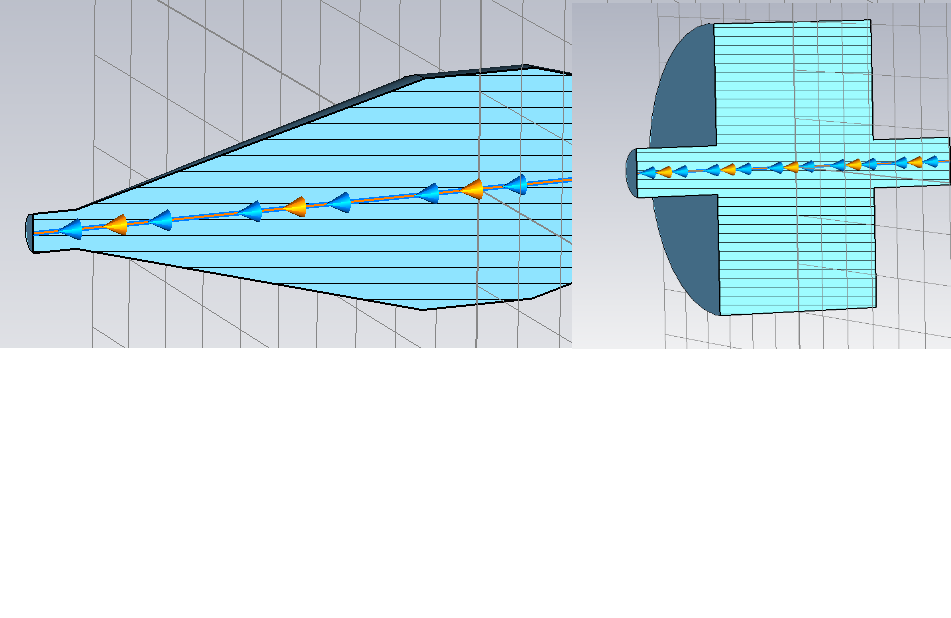
\includegraphics[width=0.45\textwidth]{Beam_Coupling_Impedance_Reduction_Techniques/figures/stepTransitionTaper.png}
\label{fig:taper_geometry}
}
\subfigure[]{
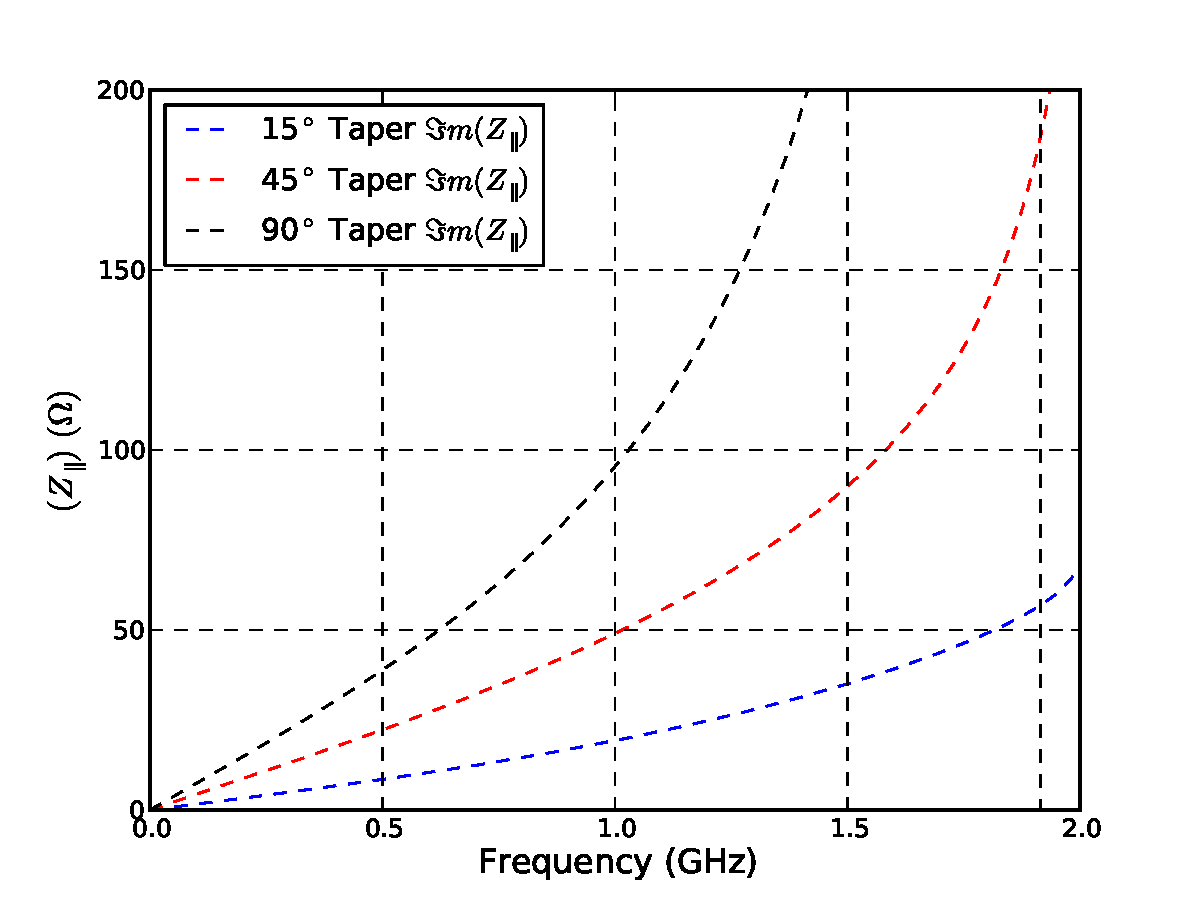
\includegraphics[width=0.45\textwidth]{Beam_Coupling_Impedance_Reduction_Techniques/figures/impedanceTaper.pdf}
\label{fig:taper_impedance}
}
\caption{An example pillbox structure with and without a tapered transition region \ref{fig:taper_geometry}, in this case with the taper at 15$^{\circ}$. The resulting imaginary component of the longitudinal impedances are shown in \ref{fig:taper_impedance}, as these are the most significant for beam stability.}
\label{fig:taper_ex}
\end{figure}

